% ============================================================================
% Calibrated Benchmarking of LLMs in Regulated Domains
% An Automated IRT Framework for Biopharma Compliance
%
% Generic arXiv preprint scaffold. Compile:
%   pdflatex main && bibtex main && pdflatex main && pdflatex main
% Figures are produced by paper/figures/gen_fig*.py (matplotlib, no LaTeX dep).
% ============================================================================
\documentclass[11pt]{article}

\usepackage[margin=1in]{geometry}
\usepackage{amsmath,amssymb}
\usepackage{graphicx}
\usepackage{booktabs}
\usepackage{xcolor}
\usepackage{enumitem}
\usepackage[numbers,sort&compress]{natbib}
\usepackage[colorlinks=true,linkcolor=blue,citecolor=blue,urlcolor=blue]{hyperref}

\graphicspath{{figures/}}

% Convenience macros
\newcommand{\todo}[1]{\textcolor{red}{[TODO: #1]}}

\title{Calibrated Benchmarking of Large Language Models in Regulated
Domains: An Automated Item-Response-Theory Framework for Biopharma
Compliance}

\author{%
  \todo{Author Name(s)} \\
  \todo{Affiliation} \\
  \texttt{\todo{email}}
}

\date{\today}

\begin{document}
\maketitle

\begin{abstract}
% Abstract — Part 1 focus (the instrument), with a one-line pointer to Part 2.
Evaluating large language models (LLMs) in regulated domains such as
biopharmaceutical compliance demands more than an aggregate accuracy
score: stakeholders need to know \emph{how hard} each question is and
\emph{where} a given system sits on a difficulty scale. We present an
automated pipeline that constructs a difficulty-calibrated question bank
for biopharma regulatory knowledge (FDA 21~CFR~Part~11, GCP, GMP,
promotional review, and informed consent) and calibrates it with
item-response theory (IRT). The pipeline (i)~generates compliance
scenarios under a ``Red Herring + subtle violation'' mandate that forces
genuine difficulty, (ii)~administers each item to a population of
synthetic AI examinees spanning models, sampling temperatures, and
system-prompt strictness, (iii)~grades responses with a dual-mode
LLM-as-judge, and (iv)~fits a Rasch (1PL) model, anchored to a fixed
baseline examinee, with classical item-fit quality control. Starting from
1{,}823 candidate items we freeze a healthy bank of
\textbf{1{,}284} items with calibrated difficulties spanning roughly
$\pm 4$ logits. A parallel track grounded in real FDA warning letters
confirms that enforced violations are systematically harder than
synthetic ones. In a second part, we treat the calibrated ability
$\theta$ as an \emph{optimization metric} and show that system-prompt
``strictness'' decomposes into a citation-\emph{format} effect and a
genuine \emph{reasoning} effect, which we separate with a strict/lenient
dual-judge design. We discuss the limits of a closed,
LLM-generated-and-judged evaluation loop and outline what external
validation would require. \todo{Tighten final numbers once py-irt
posterior SEs are wired in.}

\end{abstract}

\section{Introduction}
\label{sec:intro}

% Motivation: why calibrated difficulty (not accuracy %) matters in GxP.
Large language models are increasingly proposed as assistants in
GxP-regulated environments such as drug manufacturing, clinical trials,
and regulatory submissions. In these settings an incorrect compliance
determination carries legal and patient-safety consequences. However, the
dominant way we measure LLM competence is a single accuracy percentage on
a fixed test set, and that measure is poorly suited to this setting.
Accuracy conflates easy and hard items, it gives no per-item difficulty,
and it cannot place a new system on a stable scale for comparison across
time or across interventions.

% Gap.
Educational measurement solved an analogous problem decades ago with
\emph{item response theory} (IRT), which separates item difficulty ($b$)
from examinee ability ($\theta$) on a common latent scale
\citep{lord1980,rasch1960}. IRT is standard for human high-stakes
testing, but it is rarely applied to LLM evaluation. Where it is applied,
the usual approach is to fit IRT to an item set that already exists,
either a repurposed human exam or an established NLP benchmark. That
approach is not available here. In a specialized regulatory domain there
is no large pool of human test-takers to calibrate against, and
crowd-sourced items lack the domain subtlety that makes compliance
questions hard.

% Contributions.
This paper builds a difficulty-calibrated compliance item bank end to
end, uses it as a measuring instrument, and then tests the instrument
itself. The contributions are the following.

\begin{enumerate}[leftmargin=1.4em]
  \item \textbf{Automated item generation with a difficulty mandate.}
  I generate compliance scenarios under an explicit ``Red Herring plus
  subtle violation'' construction (Section~\ref{sec:itemgen}). Every hard
  item must contain a compliant-but-suspicious element designed to
  mislead, and the true violation must be a procedural or data-integrity
  subtlety rather than an obvious lapse. A parallel track converts real
  FDA warning letters into items, which grounds the synthetic bank in
  actual enforcement.

  \item \textbf{IRT calibration with a synthetic examinee population.}
  Lacking human test-takers, I administer each item to a population of
  synthetic AI examinees and estimate difficulty from their response
  pattern (Sections~\ref{sec:calibration}--\ref{sec:pipeline}). I fit a
  Rasch (1PL) model, anchor it to a fixed baseline examinee, and apply
  classical item-fit quality control to freeze a healthy bank of
  \textbf{1{,}284} items.

  \item \textbf{$\theta$ as an optimization metric, with a
  format-versus-reasoning decomposition.} Treating the calibrated bank as
  a fixed instrument, I measure how far two kinds of intervention move a
  model's ability: system-prompt strictness
  (Section~\ref{sec:deltatheta}) and agent architecture, including
  retrieval, self-critique, and step decomposition
  (Section~\ref{sec:phase3b}). Grading the same responses with a strict
  judge and a lenient judge separates the gain that comes from
  \emph{citation format} from the gain that reflects genuine
  \emph{compliance reasoning}.

  \item \textbf{Validation of the instrument.} Because every result rests
  on an LLM judge, I audit that judge against two independent evaluation
  frameworks (Section~\ref{sec:judgeaudit}), and I document the
  human expert-review protocol now collecting labels
  (Section~\ref{sec:expertreview}).
\end{enumerate}

The paper has three parts. Part~1
(Sections~\ref{sec:itemgen}--\ref{sec:results}) builds the
\emph{instrument} and describes what the calibrated bank looks like.
Part~2 (Sections~\ref{sec:deltatheta}--\ref{sec:phase3b}) runs two
\emph{experiments} on that instrument. Part~3
(Sections~\ref{sec:judgeaudit}--\ref{sec:expertreview}) turns the
question around and asks how far the instrument itself can be trusted.
The loop is closed, in that the same model family generates, answers, and
judges the items, and I return to what that costs in
Section~\ref{sec:discussion}.

\section{Related Work}
\label{sec:related}

\paragraph{LLM benchmarks.}
General-purpose benchmarks such as MMLU \citep{hendrycks2021mmlu},
HellaSwag \citep{zellers2019hellaswag}, and BIG-Bench
\citep{srivastava2023bigbench} report aggregate accuracy over large,
static item sets. They are invaluable for coarse ranking but do not
provide per-item difficulty parameters, standard errors, or a latent
scale on which to compare interventions. \todo{Add 1--2 domain-specific
medical/regulatory benchmarks for contrast.}

\paragraph{IRT for evaluating machines.}
A growing line of work applies item-response theory to model evaluation,
using IRT to identify informative items, to weight benchmark scores, and
to compare systems on a latent ability scale
\citep[e.g.][]{lalor2019pyirt}. \todo{Cite the specific
``IRT-for-NLP-evaluation'' papers you want to position against; note
whether they reuse human exams vs. build machine-native instruments.}
Our work differs in that the items are \emph{generated and calibrated for
machine examinees} in a domain with no human calibration pool, and the
difficulty mandate is built into generation.

\paragraph{IRT in educational measurement.}
The Rasch (1PL) model \citep{rasch1960} and the broader IRT family
\citep{lord1980} are the foundation of modern high-stakes testing.
We adopt Rasch for its specific objectivity---ability differences are
invariant to which items are used---which is precisely the property we
need when comparing $\theta$ across prompt interventions
(Section~\ref{sec:deltatheta}). We use the \texttt{girth} library
\citep{girth} for marginal-maximum-likelihood estimation and
\texttt{py-irt} \citep{lalor2019pyirt} for posterior uncertainty.

\paragraph{LLM-as-judge.}
Using a strong LLM to grade open-ended responses is now common practice
\citep{zheng2023judge}. We adopt it out of necessity---there is no human
grading pool---and mitigate its known biases with a domain-specific
rubric and a strict/lenient dual-judge design
(Section~\ref{sec:itemgen}). We treat judge error as a measured quantity
rather than assuming it away (Section~\ref{sec:discussion}).

\section{Item Generation}
\label{sec:itemgen}

% Part 1 begins: the instrument.
The bank is built from two sources: LLM-generated synthetic scenarios and
items extracted from real FDA warning letters. Both share a common schema
and are calibrated identically.

\subsection{Item schema}
Each item is a JSON record with the fields in Table~\ref{tab:schema}.
The \texttt{gold\_standard} is the reference answer used by the judge; for
hard items it must name the controlling regulation at the section level
and, where a Red Herring is present, briefly explain why it is
\emph{not} the violation.

\begin{table}[t]
\centering
\small
\begin{tabular}{@{}ll@{}}
\toprule
field & description \\
\midrule
\texttt{task\_id}      & stable identifier, e.g. \texttt{TASK-21CFR11-A1B2C3D4} \\
\texttt{domain}        & regulatory domain key (see \S\ref{sec:domains}) \\
\texttt{context}       & 4--6 sentence scenario, named fictional company \\
\texttt{question}      & single-answer compliance question \\
\texttt{gold\_standard}& reference answer + section-level citation \\
\texttt{source\_type}  & \texttt{synthetic} or \texttt{real} \\
\texttt{source\_ref}   & URL of the FDA letter (real items only) \\
\bottomrule
\end{tabular}
\caption{Item schema. \texttt{source\_type} tags the provenance track.}
\label{tab:schema}
\end{table}

\subsection{Domains}
\label{sec:domains}
Hard synthetic items cover five regulatory domains---21~CFR~Part~11
\citep{fda21cfr11} (electronic records and signatures), GCP protocol deviations,
promotional-material review, GMP manufacturing deviations, and informed
consent---plus ten \emph{targeted} 21~CFR~Part~11 sub-domains
(hybrid paper/electronic systems, legacy-system validation, audit-trail
completeness, electronic-signature components, and predicate-rule
interplay). Five parallel ``easy'' domains generate deliberately
unambiguous items used to anchor the low-difficulty end of the scale.

\subsection{The Red Herring + subtle violation mandate}
The central design decision is that hard items must be \emph{genuinely}
hard, not merely confusing. The generation prompt enforces two
constraints:
\begin{enumerate}[leftmargin=1.4em,topsep=2pt]
  \item \textbf{Red Herring.} At least one process or element that
  \emph{appears} non-compliant but is in fact fully compliant (e.g.\ a
  legacy system correctly operating read-only, a delayed-but-permissible
  timestamp). It is meant to pull the solver toward flagging a
  non-violation.
  \item \textbf{Subtle violation.} The actual gap must be a procedural
  lapse, a signature-timing issue, or a system-to-system data-integrity
  gap---never a blatant non-compliance. The common-sense answer must be
  \emph{wrong}.
\end{enumerate}
Easy items use a separate template with no Red Herring and a routine,
unambiguous violation. \todo{Add one worked hard-item example (context,
question, gold standard, and the Red Herring) as a boxed figure.}

\subsection{Real-world grounding: FDA warning letters}
A separate importer ingests FDA warning letters, extracts compliance
findings, assigns a domain, and emits items tagged
\texttt{source\_type=real}. Because these encode \emph{actual}
enforcement actions, they serve as an external check on whether the
synthetic difficulty scale is realistic; we return to this in
Section~\ref{sec:results}. \todo{State the final count of real letters
and items in this build.}

\section{Calibration with a Synthetic Examinee Population}
\label{sec:calibration}

% The 15-profile logit-b path (legacy bank pipeline), plus the bridge to
% the 45-cell Phase 1 grid used for the frozen bank.
With no human test-takers available, difficulty has to be estimated from
the responses of a \emph{synthetic} examinee population. I use two
related estimators. The first is a fast pass-rate logit used during item
generation. The second is the full Rasch fit that produces the frozen
bank, which I describe in Section~\ref{sec:pipeline}.

\subsection{Fifteen solver profiles and the pass-rate logit}
During generation, each candidate item is administered to 15 synthetic
solver profiles. The profiles span five expertise tiers (layperson,
life-sciences professional, regulatory-affairs coordinator,
regulatory-affairs specialist, and senior FDA auditor) at three sampling
temperatures each. Let $k_i$ be the number of profiles that pass item $i$
and let $\hat{P}_i = k_i / 15$ be the empirical pass rate. Under a Rasch
model in which the profile population is centered at $\theta = 0$, the
probability of a correct response to an item of difficulty $b$ is
$\sigma(\theta - b)$. So at $\theta = 0$ we have
$\hat{P}_i = \sigma(-b_i)$, and therefore

\begin{equation}
\hat{b}_i \;=\; \ln\!\left(\frac{1 - \hat{P}_i}{\hat{P}_i}\right),
\qquad \hat{P}_i \in [0.01,\, 0.99],
\label{eq:logitb}
\end{equation}

where $\hat{P}_i$ is clipped to keep $\hat{b}_i$ finite at the extremes.
Equation~\eqref{eq:logitb} ranges from $b \approx +4.6$ for a very hard
item ($\hat{P}=0.01$) to $b \approx -4.6$ for a trivially easy one
($\hat{P}=0.99$).

\subsection{Retention thresholds}
Items are retained or discarded by pass rate, as shown in
Table~\ref{tab:retention}. I widened the thresholds to $[0.05, 0.95]$ in
order to capture items that are near the extremes but still informative.

\begin{table}[t]
\centering
\small
\begin{tabular}{@{}llc@{}}
\toprule
pass rate $\hat{P}$ & outcome & retained? \\
\midrule
$\hat{P} < 0.05$        & \texttt{discarded\_too\_hard} & no \\
$0.05 \le \hat{P} \le 0.95$ & \texttt{retained}        & yes \\
$\hat{P} > 0.95$        & \texttt{retained\_easy}       & yes \\
\bottomrule
\end{tabular}
\caption{Pass-rate retention rule. Difficulty $b$ from
Eq.~\eqref{eq:logitb} is recorded for all items, including the
too-hard ones, so that they can still enter ability estimation as
failures.}
\label{tab:retention}
\end{table}

\subsection{Key assumption and its risk}
Equation~\eqref{eq:logitb} assumes that the synthetic population is
centered at $\theta = 0$. This assumption carries a risk. If the profiles
lean expert on average ($\bar{\theta} > 0$), then $b$ is biased downward
and the items look easier than they really are. Also, the 15 profiles are
highly correlated. They are the same base model run under different
prompts and temperatures, so they are not 15 independent test-takers. The
full Rasch fit in Section~\ref{sec:pipeline} relaxes the
centered-population assumption, because it estimates examinee abilities
jointly and anchors them to a fixed baseline. The remaining independence
problem is discussed in Section~\ref{sec:discussion}.

\section{The Calibration Pipeline}
\label{sec:pipeline}

The frozen bank is produced by a two-phase pipeline. Phase~1 reads the
generated items, administers them to a grid of synthetic examinees, and
fits Rasch. Phase~2 refits and applies item-fit quality control.

\subsection{Phase 1: the examinee grid}
Phase~1 builds a $3 \times 5 \times 3 = 45$-cell grid of virtual
examinees. The three factors are base model
(\texttt{llama-3.3-70b-versatile}, \texttt{openai/gpt-oss-20b}, and
\texttt{llama-3.1-8b-instant}), sampling temperature
($0.1, 0.4, 0.7, 1.0, 1.2$), and system-prompt strictness
(\texttt{none}, \texttt{neutral}, \texttt{strict}). Every
(examinee~$\times$~item) pair is administered once and graded, which
yields a binary response matrix. On $1{,}823$ items this comes to
$82{,}035$ graded attempts. Each cell is a single zero-shot call, the run
is resumable, and one audit row is written per pair.

\subsection{The dual-mode judge}
Responses are graded by an LLM judge in one of two modes. The
\emph{strict} judge, used for hard and real items, requires the correct
compliant or non-compliant conclusion \emph{and} a section-level citation
such as ``21~CFR~11.10(e)''. The \emph{lenient} judge, used for easy
items, requires only the correct conclusion and consistent reasoning,
with no citation. The lenient mode is necessary because without it the
easy items would be failed by weak examinees that never cite sections,
which would collapse the low-difficulty anchor. All judge errors are
mapped to a failing score, so that no exception escapes the matrix.

\subsection{Rasch fit and baseline anchoring}
I fit a 1PL Rasch model by marginal maximum likelihood
(\texttt{girth.rasch\_mml}; \citealp{girth}), with discrimination fixed
at $a = 1$ for all items. Difficulty is identified only up to an additive constant, so the
scale has to be anchored. In the 1PL model
$P(\text{correct}\mid\theta,b)=\sigma(\theta-b)$, so shifting every $b$
by a constant $c$ shifts every $\theta$ by $-c$. I choose
$c = \hat{\theta}_{\text{base}}$, the MLE ability of a designated
baseline examinee (\texttt{llama-3.1-8b-instant}, $t{=}0.1$, strictness
\texttt{none}). The baseline then sits at $\theta = 0$ by construction,
and all reported $b$ values are on that scale.

\subsection{Phase 2: classical item-fit quality control}
Phase~2 refits Rasch on the Phase~1 matrix and drops any item that fails
one of four classical checks.

\begin{enumerate}[leftmargin=1.4em,topsep=2pt]
  \item \textbf{Zero variance.} All-pass or all-fail items carry no
  information and their difficulty is undefined at the bound. These are
  dropped unconditionally.
  \item \textbf{Point-biserial} (corrected, item versus rest-of-total).
  A non-positive correlation means that stronger examinees do
  \emph{worse} on the item, which signals a broken gold standard. These
  are dropped at $\le 0$.
  \item \textbf{Infit} (information-weighted mean-square residual),
  dropped above $1.5$.
  \item \textbf{Outfit} (unweighted mean-square residual), dropped above
  $2.0$.
\end{enumerate}

The fit thresholds are deliberately asymmetric, with upper bounds only.
Linacre's conventional bands \citep{linacre2002infit} treat mean-squares
in $[0.5, 1.5]$ as productive for measurement, $1.5$ to $2.0$ as
unproductive but not degrading, and above $2.0$ as degrading. That
symmetric guidance is calibrated for thousands of examinees. On a 45-cell
grid, an item with a very low mean-square is a clean separator that I
want to keep, not a defect. Outfit gets the looser bound ($2.0$ against
infit's $1.5$) because it is unweighted, so a single anomalous cell at
extreme $\theta$ inflates it disproportionately on a small grid.

\paragraph{Why Rasch and not 2PL.}
A 2PL model is not identifiable on a 45-examinee grid. Marginal MLE
pinned every discrimination at the optimizer's upper bound, and joint
MLE, although it gives a real spread, is statistically inconsistent as
the number of items grows with the number of examinees held fixed. That
is exactly the regime here. Rasch is identifiable, it gives the specific
objectivity that the $\Delta\theta$ comparisons in
Section~\ref{sec:deltatheta} rely on, and it matches the model used
during generation. I retain the 2PL machinery for a future
re-evaluation, once the examinee count grows.

\section{The Frozen Bank}
\label{sec:results}

\subsection{Bank composition and quality}
Quality control reduces the $1{,}823$ input items to a frozen healthy
bank of \textbf{1{,}284} items (Table~\ref{tab:qc}). The four drop
reasons account for 539 removed items; zero-variance and non-positive
point-biserial dominate, with relatively few items failing the fit
bounds.

\begin{table}[t]
\centering
\small
\begin{tabular}{@{}lr@{}}
\toprule
stage / reason & items \\
\midrule
input items                 & $1{,}823$ \\
\quad dropped: zero-variance        & 308 \\
\quad dropped: point-biserial $\le 0$ & 155 \\
\quad dropped: infit $> 1.5$        & 14 \\
\quad dropped: outfit $> 2.0$       & 62 \\
\midrule
\textbf{frozen (healthy)}   & \textbf{1{,}284} \\
\bottomrule
\end{tabular}
\caption{Phase~2 quality-control funnel. Retention $\approx 70\%$.}
\label{tab:qc}
\end{table}

The healthy bank has median difficulty $b = +1.65$, median point-biserial
$+0.42$, median infit $0.87$, and median outfit $0.66$
(Table~\ref{tab:quality}). Difficulty spans roughly $\pm 4$ logits
(Figure~\ref{fig:bhist}); the item-fit cloud sits comfortably inside the
QC bounds (Figure~\ref{fig:itemfit}).

\begin{table}[t]
\centering
\small
\begin{tabular}{@{}lcccc@{}}
\toprule
 & $b$ & point-biserial & infit & outfit \\
\midrule
median (healthy bank) & $+1.65$ & $+0.42$ & $0.87$ & $0.66$ \\
\bottomrule
\end{tabular}
\caption{Healthy-bank summary statistics ($n = 1{,}284$).}
\label{tab:quality}
\end{table}

\paragraph{Difficulty with uncertainty.}
We report difficulty as $b \pm \mathrm{SE}$. The standard error shown
here is the analytic delta-method value for a single-item logit
difficulty,
$\mathrm{SE}(b) = 1/\sqrt{N\,P(1-P)}$ with $N = 45$ and
$P = \sigma(-b)$. This is an interim estimate; the posterior standard
deviation from a variational Rasch fit (\texttt{py-irt}) is the intended
final uncertainty and is wired into the pipeline
(\texttt{evaluator/pyirt\_fit.py}) but requires regenerating the raw
response matrix; we report the analytic value here and treat the
posterior comparison as future work (Section~\ref{sec:discussion}).

\begin{figure}[t]
\centering
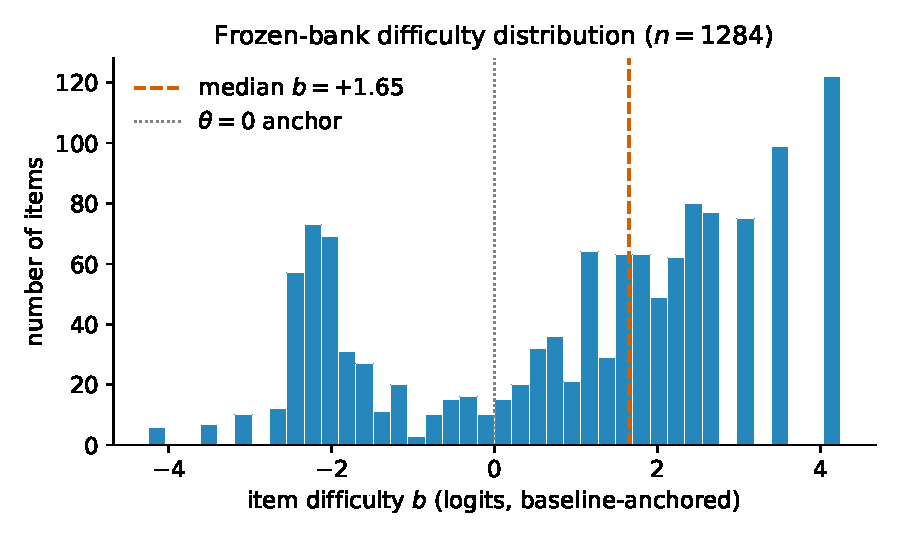
\includegraphics[width=0.78\linewidth]{fig1_b_hist.pdf}
\caption{Difficulty distribution of the frozen bank ($n = 1{,}284$),
baseline-anchored to $\theta = 0$. Median $b = +1.65$.}
\label{fig:bhist}
\end{figure}

\begin{figure}[t]
\centering
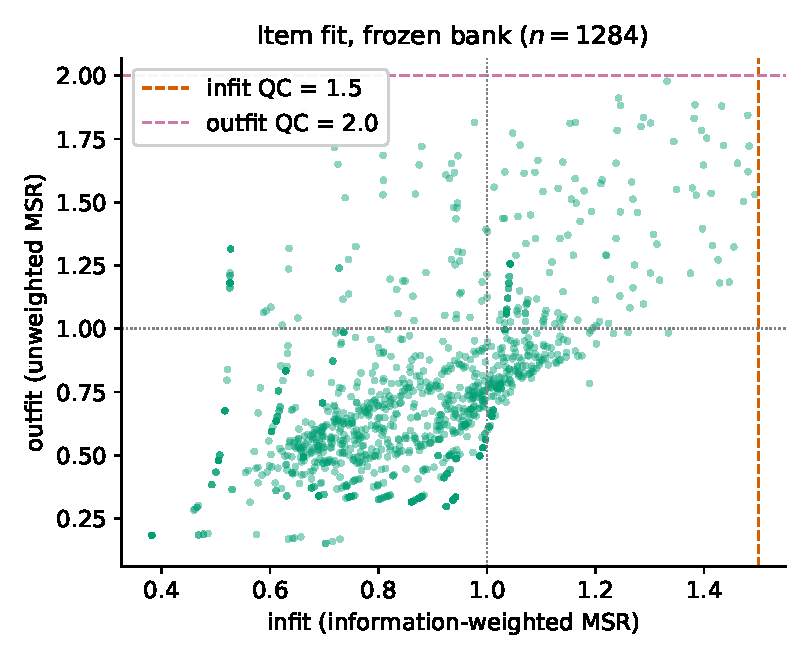
\includegraphics[width=0.62\linewidth]{fig2_item_fit.pdf}
\caption{Item fit (infit vs.\ outfit) for the frozen bank. Dashed lines
are the QC upper bounds (infit $1.5$, outfit $2.0$); dotted lines mark
the ideal Rasch value of $1.0$.}
\label{fig:itemfit}
\end{figure}

\subsection{Real-vs-synthetic difficulty gap}
Items extracted from FDA warning letters are systematically harder than
synthetic items on the frozen bank: $n = 93$ real items with mean
$b = +1.98$ versus $n = 1{,}191$ synthetic with mean $b = +1.04$, a gap
of $+0.94$ logits. A tie-corrected Mann--Whitney $U$ test confirms the
shift is not attributable to chance ($U = 66{,}516$, $z = -3.24$,
two-sided $p = 0.0012$). The effect is real but modest in magnitude:
Cliff's $\delta = +0.20$, i.e.\ a randomly drawn real item is harder than
a randomly drawn synthetic one about $60\%$ of the time. The difference
is better described as a shift in the \emph{lower tail} than a wholesale
separation: only $5$ of $93$ real items ($5.4\%$) fall below $b = 0$,
against $372$ of $1{,}191$ synthetic items ($31.2\%$), and the easiest
real item ($b = -2.00$) is still far above the easiest synthetic one
($b = -4.25$). Enforcement, in other words, rarely produces easy
questions --- but it does not produce exclusively hard ones either.

On the full Phase~1 pre-QC set ($n = 105$ real, $n = 1{,}718$ synthetic)
the mean gap is $+0.49$ logits, suggesting QC preferentially removes
easy-or-inverted synthetic items and thus sharpens the real-vs-synthetic
separation. The test is reproducible from the committed frozen bank with
no API calls via \texttt{scripts/real\_vs\_synthetic\_test.py}.

\section{Part 2 --- $\theta$ as an Optimization Metric}
\label{sec:deltatheta}

% The engineering arc: use the frozen instrument to measure interventions.
Part~1 produced a fixed, calibrated instrument. We now use it to ask an
engineering question: \emph{when a system-prompt intervention appears to
make a model ``better'' at compliance, what exactly improved?} Because
the bank is Rasch-calibrated, we can read each configuration's ability
$\theta$ on a common scale and compare interventions as differences
$\Delta\theta$.

\subsection{Setup}
We hold the bank fixed at the 1{,}284 frozen items and score nine subject
configurations: three models
(\texttt{llama-3.3-70b-versatile}, \texttt{openai/gpt-oss-20b},
\texttt{llama-3.1-8b-instant}) at a single temperature ($t = 0.4$) under
three system-prompt strictness levels (\texttt{none}, \texttt{neutral},
\texttt{strict}). Restricting the bank to the healthy subset shifts the
baseline's ability, so we re-anchor inside the analysis so that absolute
$\theta$ values remain honest; $\Delta\theta$ comparisons within a model
are invariant to this shift.

\subsection{The dual-judge decomposition}
The strict judge requires section-level citations, so a measured
``prompt effect'' can mean two very different things: the prompt taught
the model to \emph{cite} (a format unlock), or it taught the model to
\emph{reason} better about compliance. To separate them, we re-grade the
same saved responses with the lenient judge (conclusion + reasoning, no
citation) and define, per model,
\begin{align}
\text{reasoning gain} &= \Delta\theta_{\text{lenient}}
  \quad(\text{none}\!\to\!\text{strict}),\\
\text{format unlock}  &= \Delta\theta_{\text{strict}}
  - \Delta\theta_{\text{lenient}}.
\end{align}
The re-grade is offline---it reuses the response text already logged in
Phase~1---so the decomposition adds judge calls but no new solver calls.

\subsection{Results}
Under the strict judge, system-prompt strictness moves all three models,
most dramatically the 70b (Table~\ref{tab:deltatheta},
Figure~\ref{fig:deltatheta}). But the lenient judge flattens the effect
for everything except the 70b: for \texttt{gpt-oss-20b} and the 8b, the
lenient $\Delta\theta$ is essentially zero
(Figure~\ref{fig:decompose}). The honest reading is that
\textbf{system-prompt strictness primarily teaches citation format, not
compliance reasoning}---only the 70b shows a non-trivial reasoning gain
($\approx +2.5$ logits) on top of the format-unlock component.

\begin{table}[t]
\centering
\small
\begin{tabular}{@{}lcccc@{}}
\toprule
model & strict $\Delta\theta$ & lenient $\Delta\theta$
      & format unlock & reasoning gain \\
      & (none$\to$strict) & & & \\
\midrule
\texttt{llama-3.3-70b} & $+5.41$ & $+2.52$ & $+2.89$ & $+2.52$ \\
\texttt{gpt-oss-20b}   & $+0.66$ & $-0.23$ & $+0.89$ & $\approx 0$ \\
\texttt{llama-3.1-8b}  & $+1.69$ & $+0.18$ & $+1.52$ & $\approx 0$ \\
\bottomrule
\end{tabular}
\caption{Ability shift from system-prompt strictness, decomposed.
Strict $\Delta\theta$ is the headline effect; the lenient re-grade
isolates the reasoning component.}
\label{tab:deltatheta}
\end{table}

\begin{figure}[t]
\centering
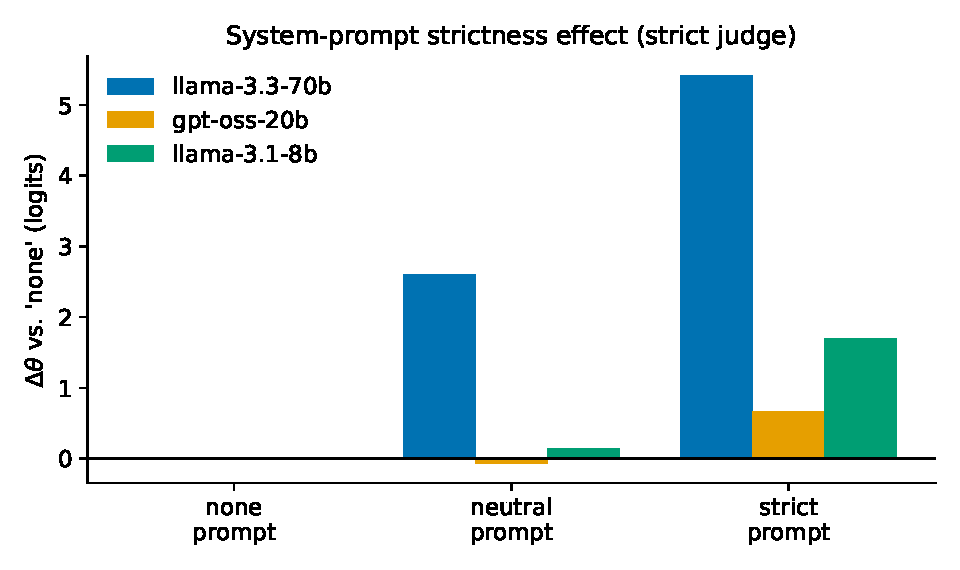
\includegraphics[width=0.82\linewidth]{fig3_delta_theta.pdf}
\caption{$\Delta\theta$ relative to the \texttt{none} prompt under the
strict judge, by model and strictness level.}
\label{fig:deltatheta}
\end{figure}

\begin{figure}[t]
\centering
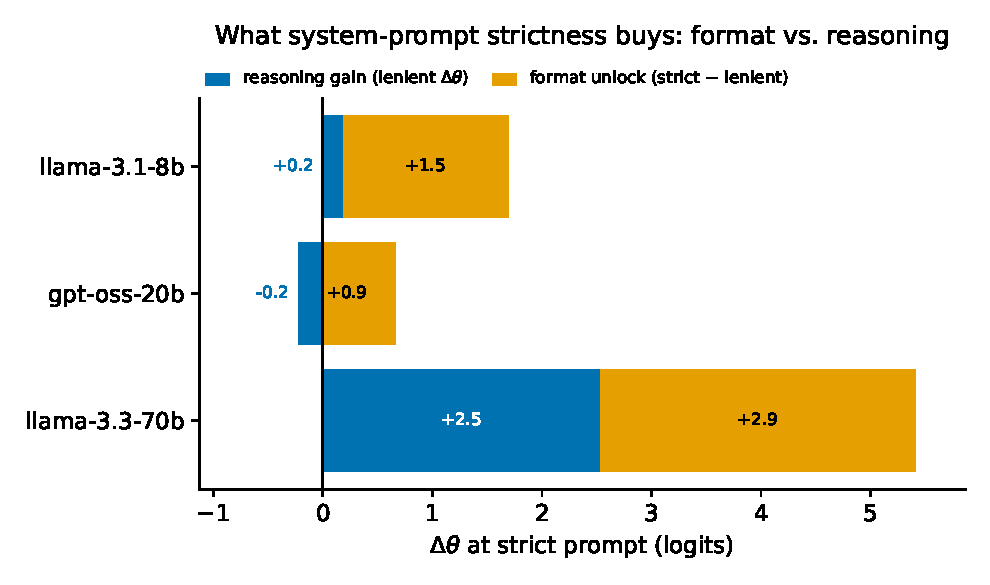
\includegraphics[width=0.86\linewidth]{fig4_decompose.pdf}
\caption{Decomposition of the strict-prompt $\Delta\theta$ into a
reasoning gain (lenient $\Delta\theta$) and a format-unlock component
(strict $-$ lenient). Only \texttt{llama-3.3-70b} shows a substantial
reasoning component.}
\label{fig:decompose}
\end{figure}

\section{Phase 3b: Architectural Interventions and Agent-Type \texorpdfstring{$\Delta\theta$}{Delta-theta}}
\label{sec:phase3b}

\subsection{Motivation}

Phase 3a established that system-prompt strictness primarily unlocks
citation \emph{format} rather than compliance \emph{reasoning}---with
only the largest model showing a genuine reasoning gain (+2.5 logits
under the lenient judge). Phase 3b tests whether \emph{structural}
changes to the agent---knowledge retrieval, self-critique, and step
decomposition---produce measurable $\Delta\theta$ beyond what prompt
engineering delivers, using the same frozen 1,284-item bank as the
measuring instrument.

\subsection{Agent Variants}

We implement three agent architectures, each a drop-in replacement for
the zero-shot baseline in the Arena runner:

\paragraph{RetrievalAgent.}
Before the single LLM call, the agent embeds the item's context and
question with the \texttt{all-MiniLM-L6-v2} sentence-transformer model
(22\,MB, local, no API call) and retrieves the top-$k$ ($k=3$) CFR
sections by cosine similarity from a pre-built numpy index covering
CFR Parts 11, 50, 58, 211 (Title 21) and Part 46 (Title 45).  The
retrieved sections are prepended to the system prompt as a
\emph{Relevant Regulations} block; all other parameters are identical
to the zero-shot baseline (same strictness level, model, temperature).
This isolates the effect of in-context regulatory grounding without
changing the agent's reasoning process.

\paragraph{CriticAgent.}
The agent makes an initial zero-shot answer, then issues a critique
prompt---``Review your previous answer for citation accuracy and
compliance determination. Correct any errors.''---and finally a
synthesis step.  With one critique round this costs three Groq calls
per item (default).  All turns share the same conversation thread so
the model has access to its own reasoning history.

\paragraph{StepDecompositionAgent.}
The agent breaks the compliance analysis into four sequential Groq
calls, each building on the prior step's output: (1)~identify the
regulated activity and parties; (2)~identify the governing CFR/ICH
provision; (3)~assess compliance or violation; (4)~state the final
determination with section-level citation.  This mirrors a structured
legal-analysis workflow and tests whether explicit chain-of-thought
scaffolding improves compliance reasoning.

\subsection{Experimental Grid}

The Phase 3b grid crosses two models (llama-3.3-70b-versatile,
llama-3.1-8b-instant) $\times$ one temperature (0.4) $\times$ two
strictness levels (none, strict) $\times$ four agent types (zero\_shot,
retrieval, critic, step\_decomp), yielding 16 examinee cells.  Every
cell is administered the full frozen 1,284-item bank, anchored to the
Phase 1 baseline ($\theta = 0$) using the same re-anchoring procedure
as Phase 3a (Section~\ref{sec:delta_theta}).

\subsection{Results}

\begin{table}[h]
\centering
\caption{Phase 3b $\Delta\theta$ by agent type relative to zero-shot baseline
         (same model, temperature, strictness). \todo{Fill after phase3b run.}}
\label{tab:phase3b}
\begin{tabular}{llcc}
\toprule
Agent type & Model & $\Delta\theta$ (strictness=none) & $\Delta\theta$ (strictness=strict) \\
\midrule
retrieval   & llama-3.3-70b & \todo{} & \todo{} \\
critic      & llama-3.3-70b & \todo{} & \todo{} \\
step\_decomp & llama-3.3-70b & \todo{} & \todo{} \\
retrieval   & llama-3.1-8b  & \todo{} & \todo{} \\
critic      & llama-3.1-8b  & \todo{} & \todo{} \\
step\_decomp & llama-3.1-8b  & \todo{} & \todo{} \\
\bottomrule
\end{tabular}
\end{table}

\todo{Interpret Table~\ref{tab:phase3b}: does in-context CFR retrieval
move $\theta$ beyond the zero-shot baseline? Is the retrieval gain
larger under strict (citation-requiring) than lenient grading---which
would suggest the agent is using the retrieved sections for format
rather than reasoning? Does step decomposition produce a consistent
reasoning gain across model sizes?}

\section{Discussion and Limitations}
\label{sec:discussion}

We are deliberately explicit about what this instrument is and is not.

\paragraph{The evaluation loop is closed.}
The same model family generates items, answers them, and judges the
answers. Any systematic blind spot---a regulatory nuance the model
family consistently misreads---is invisible to the loop and can poison
both the gold standard and its grading. The real-FDA track partly
mitigates this by injecting externally authored content, but the judge is
still an LLM. External validity against human expert judgment is unproven.

\paragraph{Synthetic examinees are correlated, not independent.}
Classical IRT calibration assumes many independent test-takers
(hundreds to thousands). Our 45-cell grid is three base models under
prompt and temperature variation; cells sharing a base model are highly
correlated. This makes the difficulty estimates more informative than a
two-profile design but less trustworthy than the examinee count alone
would suggest. Standard errors should be read in that light.

\paragraph{Difficulty uncertainty is currently analytic.}
The $b \pm \mathrm{SE}$ reported in Section~\ref{sec:results} uses an
analytic single-item logit SE. The intended final uncertainty is the
posterior standard deviation from a variational Rasch fit
(\texttt{py-irt}), which is implemented but requires regenerating the raw
response matrix. We expect the posterior SDs to be \emph{wider} than the
analytic values, given only 45 examinees---which is the honest message,
not a defect to hide. \todo{Report the py-irt posterior SDs once
regenerated and compare to the analytic SE.}

\paragraph{Judge error is real and measured.}
Re-grading introduced a measurable judge-error rate (failed judge calls
mapped to a failing score). We treat this as part of the measurement
noise rather than assuming it away, but a human-validated subset would be
needed to quantify judge bias as opposed to judge variance.

\paragraph{What would make this credible as measurement.}
Three things, in priority order: (i)~\emph{human expert validation} of a
stratified sample of gold standards and verdicts, providing an external
anchor for the difficulty scale; (ii)~a formal \emph{real-vs-synthetic}
test (Mann--Whitney~$U$) on the difficulty gap reported descriptively in
Section~\ref{sec:results}; and (iii)~\emph{cross-model} examinee
expansion to reduce within-family correlation. The Red Herring mandate is
enforced at generation but not audited---no automated check verifies that
a genuine Red Herring is present and correctly explained in the gold
standard.

\paragraph{Honest framing of the contribution.}
This is a pipeline and an instrument, not a psychometric certification.
The $\Delta\theta$ decomposition (Section~\ref{sec:deltatheta}) is the
most defensible empirical result: it is a within-model comparison that is
invariant to the scale's absolute anchoring, and it delivers a concrete,
falsifiable claim---system-prompt strictness mostly buys citation format.

\section{Conclusion}
\label{sec:conclusion}

I presented an end-to-end pipeline that builds and IRT-calibrates a
difficulty-graded question bank for biopharma regulatory compliance, and
that then uses the bank as a measuring instrument.

Part~1 built the instrument. It generates hard items under a Red Herring
plus subtle-violation mandate, administers them to a synthetic examinee
population, and freezes a healthy bank of $1{,}284$ Rasch-calibrated
items spanning roughly $\pm 4$ logits. A parallel track built from FDA
warning letters gives items that are harder than the synthetic ones
($+0.94$ logits, two-sided $p = 0.0012$), although the difference is a
shift in the lower tail rather than a full separation.

Part~2 ran two experiments on that instrument. Treating the calibrated
ability $\theta$ as an optimization metric, and using a strict and a
lenient judge on identical response text, I found that system-prompt
strictness primarily unlocks citation \emph{format} rather than
compliance \emph{reasoning}, with only the largest model showing a
genuine reasoning gain. Architectural interventions, namely retrieval,
self-critique, and step decomposition, showed the same pattern. All three
raised $\theta$ under lenient scoring and lowered it under strict
scoring. So the effect is not specific to prompt editing. When a judge
enforces section-level citations, citation format dominates the
measurement scale.

Part~3 turned the question toward the instrument itself. An audit against
two independent evaluation frameworks showed that a citation-requiring
G-Eval rubric recovers my judge's verdicts at $\mathrm{AUC} = 0.838$,
while a groundedness metric performs at chance. That is the pattern the
design predicts, and it rules out the possibility that the verdicts are
arbitrary. It does not show that they are correct, because every metric
in the audit shares a base model with the judge. The expert-review
protocol described in Section~\ref{sec:expertreview} is designed to close
that gap, and its labels are being collected now.

The remaining work follows from the limitations. The analytic difficulty
SE should be replaced with \texttt{py-irt} posterior standard deviations,
the examinee population should be expanded across model families to
reduce correlation, and the Red Herring mandate should be audited rather
than merely enforced. Beyond measurement, a calibrated bank enables
adaptive item selection, meaning the choice of the item whose difficulty
best matches a system's current $\theta$, and it gives a principled way
to track whether an intervention moves regulatory reasoning on a stable
scale.

The broader point is methodological. A single accuracy number cannot
distinguish a system that reasons better from one that has learned the
grader's formatting preference. Separating item difficulty from examinee
ability makes that distinction measurable, and in this domain the
distinction turned out to matter more than the headline numbers
suggested.


\bibliographystyle{plainnat}
\bibliography{references}

\end{document}
